\documentclass[12pt,a4paper]{article}
\usepackage[margin=1in]{geometry}
\usepackage[T1]{fontenc}
\usepackage{textcomp}
\usepackage{graphicx}
\usepackage{float}
\usepackage{multirow}
\usepackage{amsmath}
\usepackage{listings}  % 添加这个
\usepackage{xcolor}     % 添加这个（可选，用于颜色）
\usepackage{tikz}
\usepackage{makecell}
\usetikzlibrary{arrows.meta}

\lstset{
    basicstyle=\ttfamily\footnotesize,         
    commentstyle=\color{gray},          
    keywordstyle=\color{blue},          
    stringstyle=\color{red},          
    numbers=left,                       
    numberstyle=\tiny,                  
    frame=single,                        
    breaklines=true,                     
    backgroundcolor=\color{gray!5},    
    linewidth=1.05\textwidth,           
    literate={"}{"}2 {'}{'}2,          
    showstringspaces=false,              
    basewidth={0.55em, 0.5em},          
    xleftmargin=0pt,                    
    xrightmargin=0pt,                   
}

\title{\textbf{\Huge COMP2016 \\Group Project Report}}
\author{\textbf{\Huge Group 5}}
\date{}

\renewcommand{\figurename}{Fig.}

\begin{document}
\maketitle
\vspace{16em}
\begin{center}
\renewcommand{\arraystretch}{1.3} 
\begin{tabular}{|c|c|}
\hline
\large Student ID & \large Name  \\
\hline
24266418 & HUANG Yenan  \\
\hline
24266949 & CHEN Zhengxian  \\
\hline
24267376 & YUE Qu \\
\hline
24267422 & LIU Shuangming  \\
\hline
\end{tabular}
\end{center}

\newpage

\section*{Database Design}
\subsection*{1. ER Diagram}
\begin{figure}[H]
    \centering
    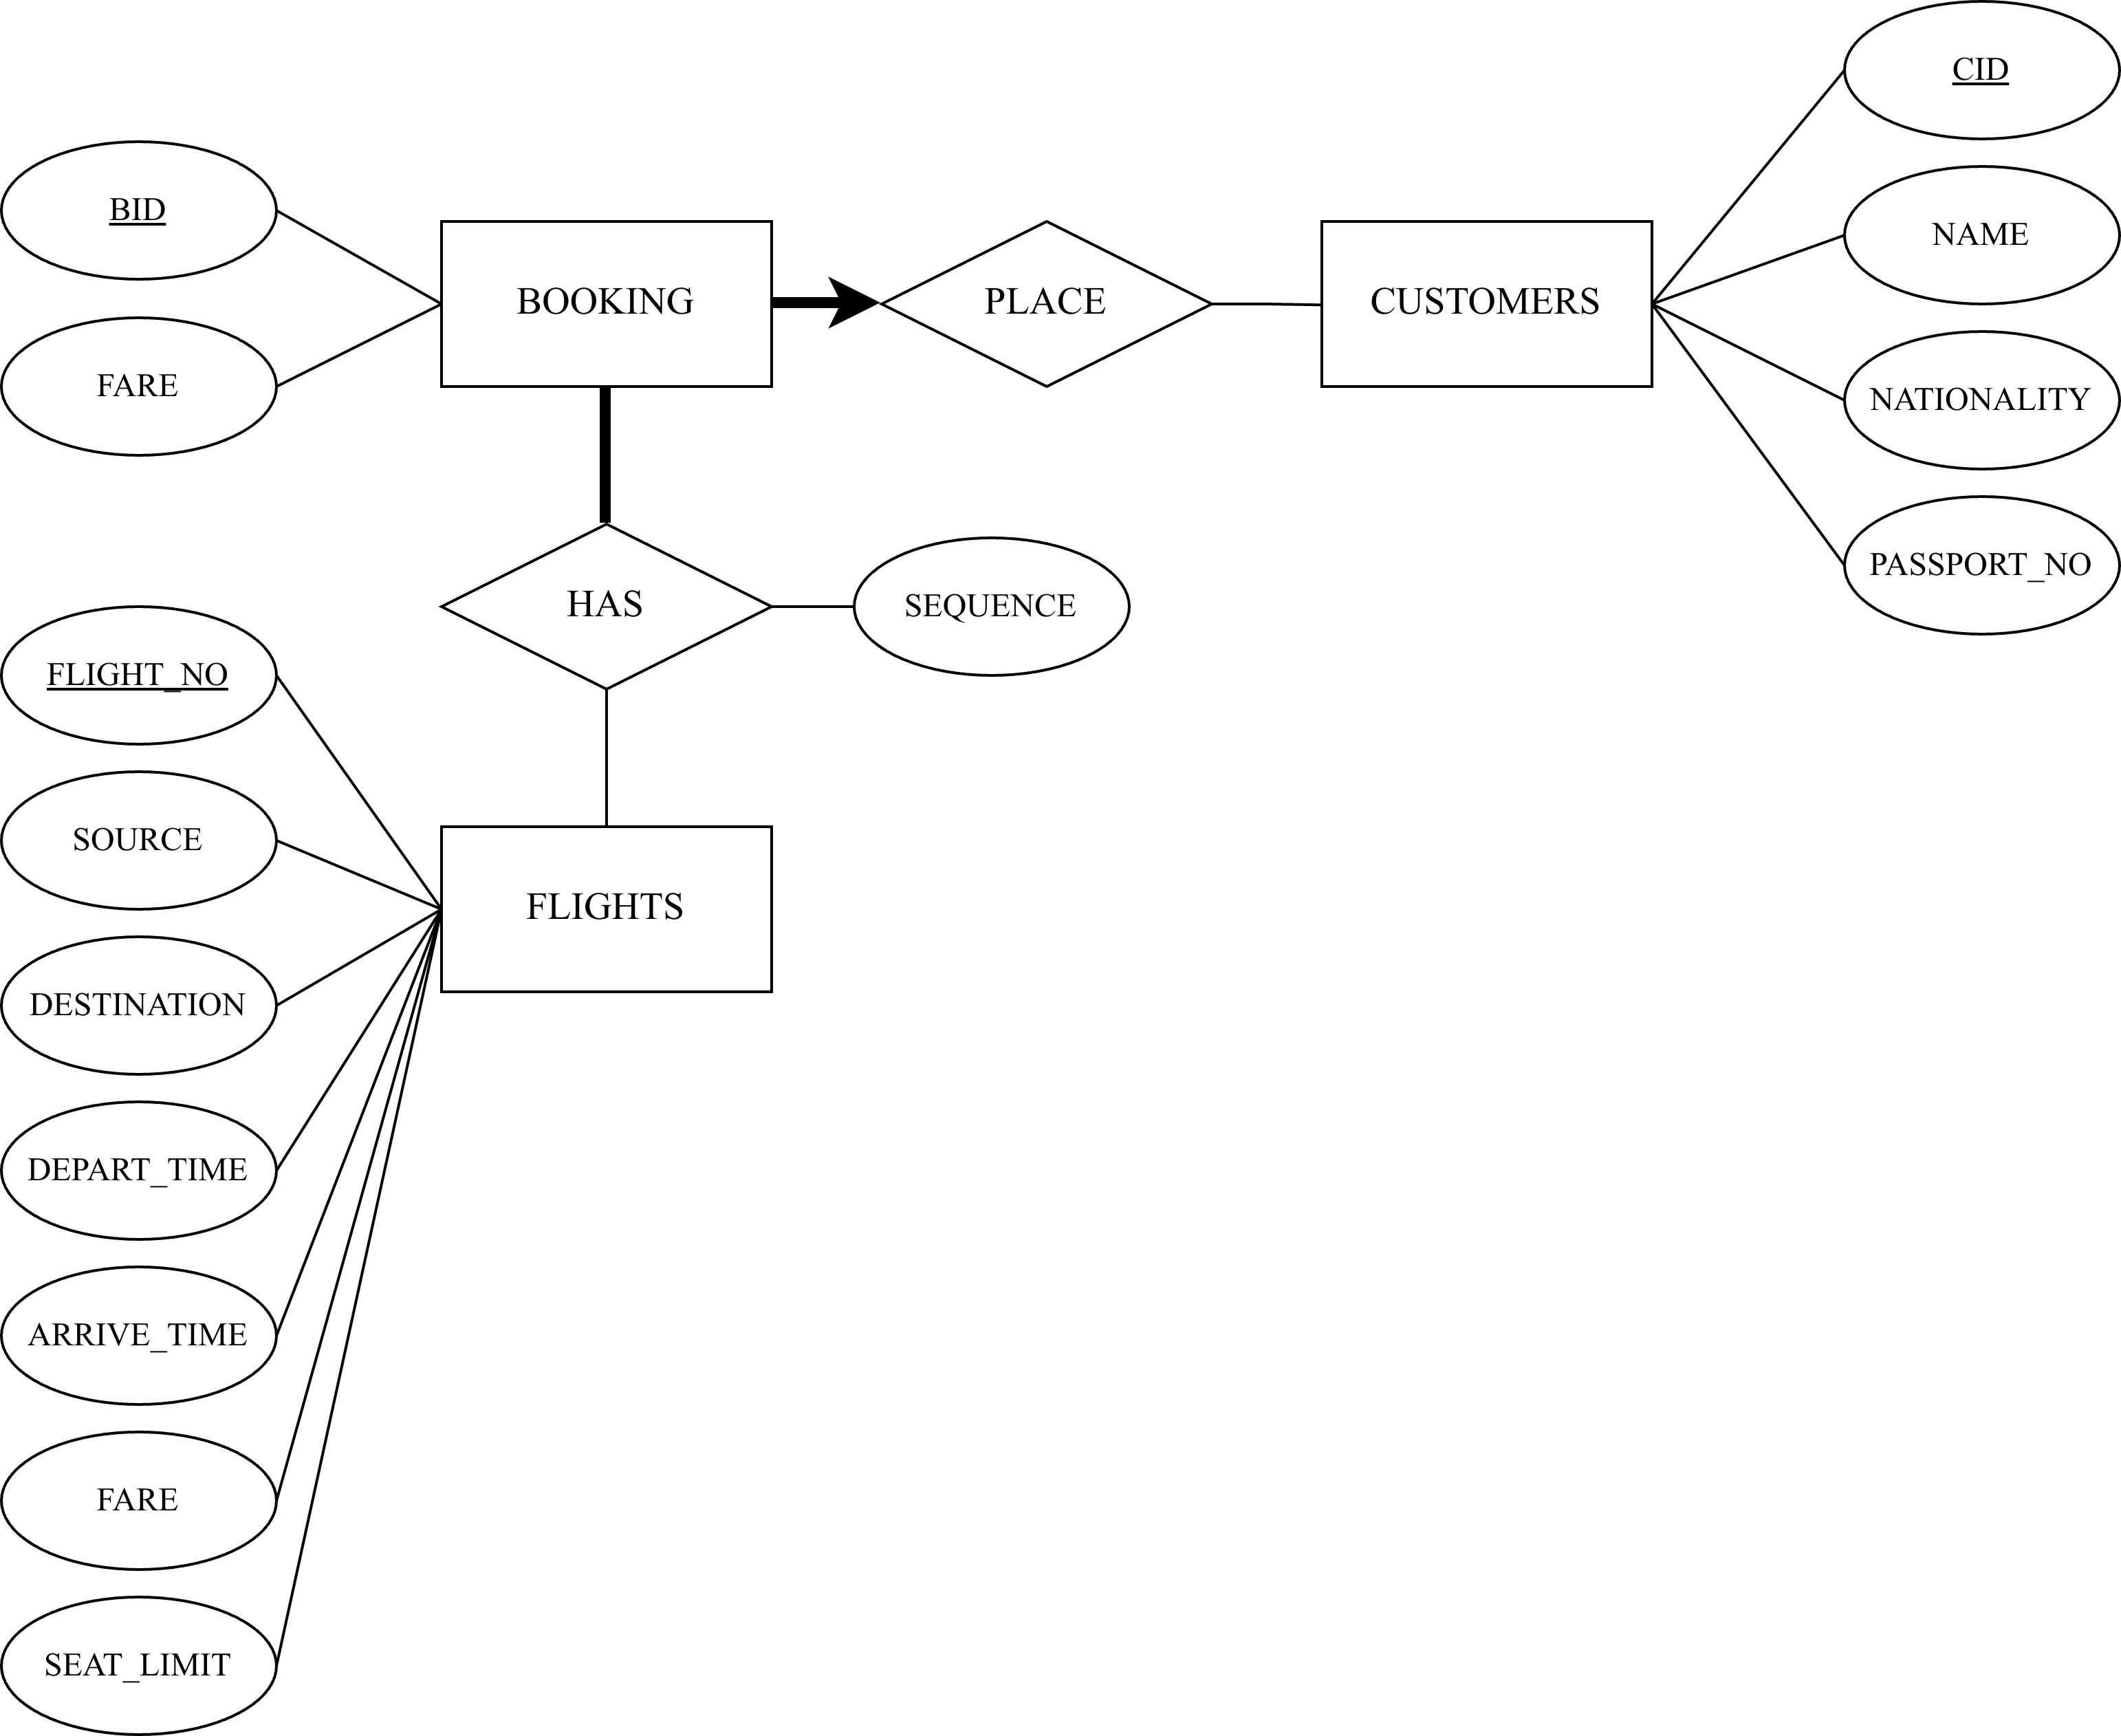
\includegraphics[width=0.8\textwidth]{ER.png}
    \caption{ER Diagram of Flight Booking System}
\end{figure}
\noindent Corresponding explanation:
\\Entity: 
\begin{itemize}
    \item \textbf{FLIGHTS}\\
    (attribute: flight\_no, source, dest, depart\_time, arrive\_time, fare, seat\_limit)\\
    Primary key: flight\_no
    \item \textbf{CUSTOMERS}\\
    (attributes: customer\_id, name, nationality, passport\_no)\\
    Primary key: customer\_id
    \item \textbf{BOOKING}\\
    (attributes: bid, derived attribute: fare)\\
    Primary key: bid
\end{itemize}
Relationships between BOOKING and FLIGHTS: HAS (attributes: sequence)\\
Relationships between BOOKING and  CUSTOMERS: PLACE
\\
1. Booking can have many flights and a flight can be included in many bookings. \\A Booking must have at least one flight, and a flight may not have any booking.\\
2. A customer can place many bookings but one booking can only be placed by one customer.\\
A booking must be placed by at least one customer and the customer may not place any bookings.

\subsection*{2. Table Designs}

\begin{center}
\footnotesize
\renewcommand{\arraystretch}{1.2}
\begin{tabular}{|l|l|l|}
\hline
\textbf{Table} & \textbf{Columns} & \textbf{Description} \\
\hline
\textbf{FLIGHTS}
& \makecell[l]{flight\_no, source, dest,\\depart\_time, arrive\_time,\\ fare, seat\_limit}
& \makecell[l]{\textbf{flight\_no} means flight number, it is a primary key.\\
\textbf{source} means the departure city.\\
\textbf{dest} means the destination city.\\
\textbf{seat\_limit} means the amount of seat in this flight.} \\
\hline
\textbf{CUSTOMERS}
& \makecell[l]{cid, cname,nationality,\\ passport}
& \makecell[l]{\textbf{cid} means customer ID, it is a primary key.\\
\textbf{cname} means customer name.\\
\textbf{passport} is unique.} \\
\hline
\textbf{BOOKING}
& \makecell[l]{bid, cid, bfare, fcount}
& \makecell[l]{\textbf{bid} means booking ID, it is a primary key.\\
\textbf{cid} is a foreign key references CUSTOMERS(cid).\\
\textbf{bfare} means total booking fare (if discount).\\
\textbf{fcount} means the amount of involved flights.} \\
\hline
\textbf{HAS}
& \makecell[l]{bid, flight\_no, fsequence}
& \makecell[l]{\textbf{(bid + flight\_no)} is primary key.\\
\textbf{bid} references BOOKING(bid).\\
\textbf{flight\_no} references FLIGHTS(flight\_no).\\
\textbf{fsequence} means the order of flight(s) in a booking.} \\
\hline
\end{tabular}
\end{center}

\subsection*{Drop Tables}
\lstinputlisting[language=SQL]{group5_dbdrop.sql}
\subsection*{Create Tables \& Constraints \& Triggers}
\lstinputlisting[language=SQL]{group5_dbinsert.sql}
\newpage
The description of tables: 
\lstinputlisting[breaklines=false]{Tables.txt}
\newpage
The result of tables after demo:
\lstinputlisting[breaklines=false]{result.txt}
\subsection*{3. Normalization}
All tables besides CUSTOMERS are all in 3\textsuperscript{rd} normal form

\vspace{1em}

CUSTOMERS:

\vspace{0.5em}

\begin{center}
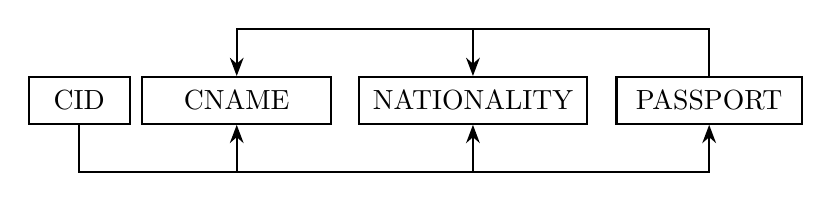
\begin{tikzpicture}[
    font=\normalsize,
    >=Stealth, thick
]

\node[draw, thick, inner xsep=9pt, inner ysep=5pt] (cid)  at (0, 0) {CID};
\node[draw, thick, inner xsep=15pt, inner ysep=5pt] (name) at (2, 0) {CNAME};
\node[draw, thick, inner xsep=5pt, inner ysep=5pt] (nat)  at (5, 0) {NATIONALITY};
\node[draw, thick, inner xsep=7pt, inner ysep=5pt] (pass) at (8, 0) {PASSPORT};

\draw[->] (cid.south) -- ++(0,-0.6) -- ++(2,0) -- (name.south);

\draw[->] (cid.south) -- ++(0,-0.6) -- ++(5,0) -- (nat.south);

\draw[->] (cid.south) -- ++(0,-0.6) -- ++(8,0) -- (pass.south);

\draw[->] (pass.north) -- ++(0,0.6) -- ++(-3,0) -- (nat.north);

\draw[->] (pass.north) -- ++(0, 0.6) -- ++(-6, 0)-- (name.north);

\end{tikzpicture}
\end{center}

Removing transitive dependency:

\vspace{0.5em}

\begin{tabular}{|c|c|}
\hline
CID & PASSPORT \\
\hline
\end{tabular}

\vspace{1em}

\begin{tabular}{|c|c|c|}
\hline
PASSPORT & CNAME & NATIONALITY \\
\hline
\end{tabular}

\vspace{1em}

\newpage
\section*{Python Code} 
\begin{table}[h]
\centering
\caption{Core Methods of Flight Management System}
\begin{tabular}{|l|p{10cm}|}
\hline
\textbf{Method}         & \textbf{Description} \\
\hline
flight\_info()          & Display detailed information of a specified flight. \\
\hline
add\_flight()           & Add a new flight record to FLIGHTS table. \\
\hline
del\_flight()           & Delete an existing flight from FLIGHTS table. \\
\hline
calculate\_fare()       & Calculate total fare (with discount) according to the number of flights. \\
\hline
search\_flight()        & Search flights based on source, destination, transfer times and maximum travel time. \\
\hline
make\_booking()         & Create a new booking for a customer and bind the selected flights. \\
\hline
cancel\_booking()       & Cancel an existing booking .\\
\hline
display\_flights\_tables() & Display all flight records. \\
\hline
\end{tabular}
\end{table}
\lstinputlisting[language=Python]{group5_source.py}

\end{document}